% Тут используется класс, установленный на сервере Papeeria. На случай, если
% текст понадобится редактировать где-то в другом месте, рядом лежит файл matmex-diploma-custom.cls
% который в момент своего создания был идентичен классу, установленному на сервере.
% Для того, чтобы им воспользоваться, замените matmex-diploma на matmex-diploma-custom
% Если вы работаете исключительно в Papeeria то мы настоятельно рекомендуем пользоваться
% классом matmex-diploma, поскольку он будет автоматически обновляться по мере внесения корректив
%

% По умолчанию используется шрифт 14 размера. Если нужен 12-й шрифт, уберите опцию [14pt]
%\documentclass[14pt]{matmex-diploma}

\documentclass[14pt]{matmex-diploma-custom}

\begin{document}
% Год, город, название университета и факультета предопределены,
% но можно и поменять.
% Если англоязычная титульная страница не нужна, то ее можно просто удалить.
\filltitle{ru}{
    chair              = {Математическое обеспечение и администрирование \\ информационных систем},
    title              = {Разработка сервиса для заказа еды},
    % Здесь указывается тип работы. Возможные значения:
    %   coursework - Курсовая работа
    %   diploma - Диплом специалиста
    %   master - Диплом магистра
    %   bachelor - Диплом бакалавра
    type               = {coursework},
    position           = {студента},
    group              = 244,
    author             = {Липаев Савелий},
    supervisorPosition = {к.\,т.\,н.,},
    supervisor         = {Литвинов Ю.\,В.},
%   university         = {Санкт-Петербургский Государственный Университет},
%   faculty            = {Математико-механический факультет},
%   city               = {Санкт-Петербург},
%   year               = {2019}
}
\maketitle
\tableofcontents

% У введения нет номера главы
\section{Введение}
    Обучаясь в любом вузе страны (или школе) студенты (ученики) должны иметь возможность правильно питаться.
    В большинстве учебных заведениях существуют столовые которые находиться в том же здании (или же рядом).
    Когда ученики приходят поесть в перерыве между занятий, возникает огромная очередь у кассы (хотя во время занятий в столовой почти не бывает посетителей).

    В результате чего многие студенты перестают посещать такие столовые, из-за нежелания тратить время в очереди, а потом есть в спешке — т.е. столовая теряет прибыль, а студент, либо остаётся голодным, либо с большой вероятностью опаздывает на следующую пару.

    Большинство современных кафе предоставляют различные приложения для предварительного заказа еды -- это позволят сократить очереди и увеличить количество посетителей. Подобное приложение адаптированное для студенческих столовых было бы очень востребовано.

\section{Постановка задачи}
    В данной семестровой были поставлены следующие задачи:
    Разработка мобильного приложение для предварительного заказа еды, на определённое время, в конкретной столовой, но без привязки к конкретному вузу.
    Написание RESTful API, обеспечивающий доступ к данным через запросы по сети и позволяющий максимально разделить фронтенд и бэкэнд, а так же увеличить производительность даже при относительно высокой нагрузке, благодаря следованию архитектурному стилю REST\cite{rest_xamarin}.
    Проектирование и реализация БД.

    Следование современным стандартам разработки ПО (Docker, swagger, CI в виде trello и appveyor, Git, Github)
    Написание веб приложения для кассиров.

\section{Обзор}
\subsection{Обзор существующих решений}

    \begin{figure}
    \centering
    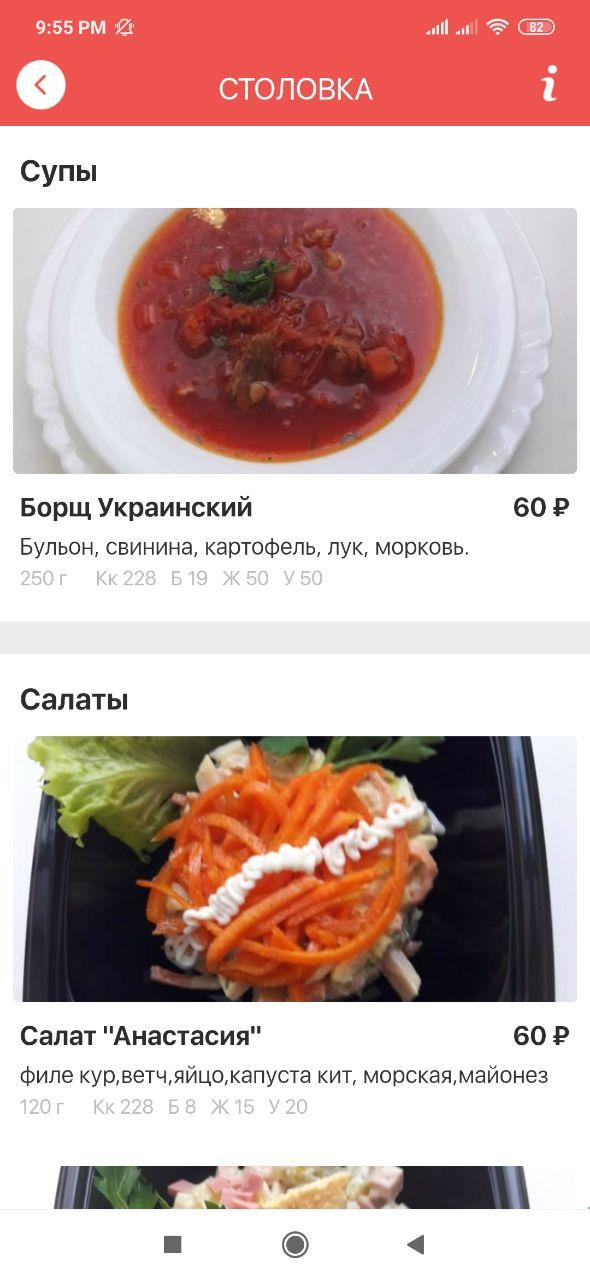
\includegraphics[scale=0.40]{fig1.jpg}
    \caption{UI Сытый офис}
    \end{figure}

    Самыми близкими аналогами являются рестораны, у которых есть возможность
    \subsection{Столовая Поварёшка}
    \begin{description}
        \item[+] Интуитивный, неперегруженный пользовательский интерфейс
        \item[—] Узко специализированный, только для одной сети
    \end{description}
	\subsection{Сытый офис}
	\begin{description}
        \item[+] Есть и веб-интерфейс и приложение для мобильных устройств
        \item[—] Сервис работает только в двух городах
        \item[—] Не адаптирован для студентов
    \end{description}
    \subsection{KFC}
	\begin{description}
        \item[+] Простой и красивый веб-интерфейс
        \item[+] Удобное мобильное приложение для iOS, Android
        \item[—] Сервис ориентирован только на сеть рестаранов KFC
    \end{description}

\section{Реализация}
    \subsection{Архитектура}
        \begin{figure}
            \centering
            \includegraphics[scale=0.40]{xamarin_forms_logic2.png}
            \caption{Xamarin.Forms App Architecture}
        \end{figure}
        В качестве основного фреймворка для написания мобильного приложения использовался Xamarin.Forms (далее XF).
        XF является отличным выбором для мультиплатформенной разработки.

        Приложение, написанное на XF имеет единую логику для всех платформ написанную на языке C\#,
        что тоже сыграло роль в выборе этого фреймворка, также он позволяет писать единый UI для всех платформ,
        но не запрещает нативной реализации всего UI или какой-то небольшой части.

        Поскольку всё компилируется в нативный код мобильных платформ, приложения высокую XF имеют высокую производительность,
        очень близкую к нативной, а иногда и выше.\footnote{Performance Comparison: Xamarin.Forms, Xamarin.iOS, Xamarin.Android vs Android and iOS \cite{perf_compar_2}}.
        В качестве архитектурного паттерна использовался Model-View-ViewModel(MVVM)\cite{MVVM_wiki},
        позволяющий разделить бизнес-логику и пользовательский интерфейс.
        MVVM является самым распространенным архитектурным паттерном для XF.

        Для авторизации в приложение использовался открытый протокол авторизации OAuth 2.0, позволяющий мобильному приложению получать ограниченный доступ к аккаунту пользователя на различных сервисах.
        В приложении возможно проходить аутентификацию через Google и ВКонтакте.

        Работает это следующим образом:
        \begin{enumerate}
            \item Приложение переадрессовывает на страницу авторизации сервиса
            \item Пользователь авторизуется и подтверждает выдачу прав
            \item Сервис переадрессовывает обратно в приложение, передавая приложению authorization code
            \item Приложение отправляет POST запрос с authorization code, в результате которого получает access token
            \item С помощью токена приложение может получить данные о пользователе, которые он сам разрешил при подтверждении выдачи прав
        \end{enumerate}

        Для работы с RESTful API использовали Refit,
        позволяющий легко описывать спецификацию в виде интерфейса с понятными выходными и входными параметрами,
        а также с возможностью манипулирования HTTP-заголовками для отдельных запросов.

        При разработке мобильных приложений нужно учитывать нестабильное соединение с сетью,
        соответственно, возникает необходимость повторного выполнения запросов,
        не перегружая пользователя дополнительными просьбами повторить действие.
        Для этого используется библиотека \textbf{Polly}\cite{polly_github}, с помощью которой удобно обрабатывать неудачные сетевые запросы.

        \subsection{ASP.NET Backend}
            \subsubsection{Jwt and Identity}
                JWT(JSON web tokens) - это стандарт для кодирования данных, который включает в себя информацию о роли пользователя и другие данные, относящиеся к вашему сайту.
                - JWT предлагает безопасный метод отправки этой информации с использованием общего секрета.
                Разные маршруты могут требовать разных ролей, с перенаправлениями на другие страницы при неудачной аутентификации.
                Это означает, что вы можете использовать закодированный.
                Роль пользователя для управления содержимым и контроля пользовательских возможностей.
    
            \subsubsection{RESTfull API}
                Для кэширования информации о пользователе использовалось хранилище Akavache\cite{akavache_github}, работающее поверх SQLite3.
                
                Стоит отметить, что для кэширования можно было использовать другие мобильные СУБД,
                например Realm, но они были не так просты в использовании как Akavache и обладали избыточной функциональностью.

    \begin{figure}
        \centering
        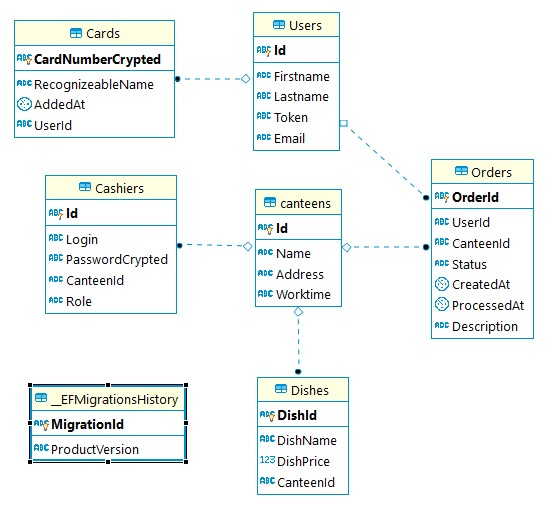
\includegraphics[scale=0.8]{database_arch1.jpg}
        \caption{База данных}
        \label{db_arch}
    \end{figure}
    Для работы с СУБД PostgreSQL на бэкенде используется Entity Framework Core,
    схема базы данных представлена на рисунке \ref{db_arch}.

    Для оптимизации запросов к RESTfull API используется кэширование с помощью mem-cache бд Redis\cite{redis_dotnet_doc}.

    3.6) EF PostgreSQL, Redis
    PostgreSQL
    3.7) Docker and CI(appveyor, travis)
        Для автоматизации тестиоования использовалмя AppVeyor и TravisCI что позволяло сразу же во время разработки получить готовую сборку, проверенную с помощью юнит-тестов
    3.8) Vue.js -- не готово!!!
    
    3.9) Swagger
    Проблема в том, что REST не является само описательным протоколом.
    Это значит, что клиент должен знать конкретную комбинацию URL, HTTP метода и формата ответа.
    В некоторых случаях необходимо также знать также формат тела запроса.
    В любом случае, REST endpoints всегда должны быть описаны в одном конкретном документе, доступном для всех остальных разработчиков.
    Но Swagger — это не просто спецификация. Основная его мощь заключается в дополнительных инструментах.
\section{Результаты}

\begin{enumerate}
    \item Получен опыт работы с фреймворком для создания мобильных приложени Xamarin.Forms
    \item Разработано Мобильное приложение для заказа еды
    \item Написан RESTfull API для получения данных
    \item Реализованна схева авторизации пользователей с помощью протокола OAuth 2.0
    \item Опыт работы с IdentityServer для ASP.NET
    \item Получен опыт прототипирования интерфейса мобильного приложения
    \item Получен опыт использования СУБД PostgreSQL, в связке с Redis, ORM EF
    \item Опыт настройки веб сервера + devops(docker,ci,deploy)
\end{enumerate}

\nocite{*}
\bibliographystyle{ugost2008ls}
\bibliography{diploma.bib}
\end{document}
